On notera par la suite gmresRES notre algortihme de gmres redémarré, et gmresMRES le gmres redémarré de matlab. On notera aussi gmresM le gmres de matlab, sans redémarrage.

\subsection{Test sur le préconditionnement des matrices}
On effectue un premier test sur la matrice $hor\_131$ en changeant le préconditionnement. On choisit cette matrice car elle est de base mal conditionnée ($cond(A) = 1.337e+5$), et ses valeurs propres semblent éloignées les unes des autres : on sait alors que la norme du résidu risque de ne pas décroitre trés vite, et que que le nombre d'itération sera surement important. On fixe $maxit = 600$ et $tol = 1e-6$. 
\subsubsection*{Sans préconditionnement}

gmresRES et gmresM ont un résidu 8.27e-1, et ne convergent pas. dqgmres a un résidu de 7.04e-1 et ne converge pas. gmresM a un résidu de 5.65e-07 et converge. Voici le tracé logarithmique des résidus en fonction de l'itération j :
\begin{center}
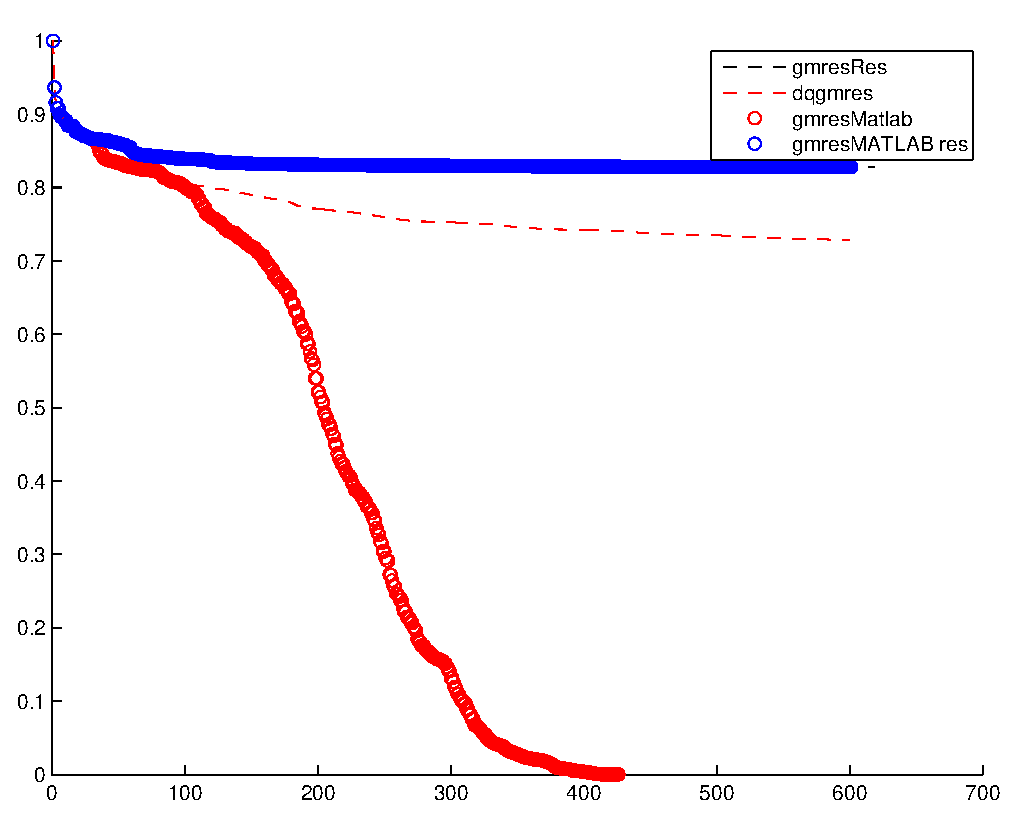
\includegraphics[scale=0.65]{sanspre.eps}
\end{center}

\subsubsection*{Avec préconditionnement diagonal}
On prend M1 qui vaut l'identité et M2 qui vaut la diagonale de A. Cette fois tous les algorithmes convergent. gmresRES a un résidu de 3.32e-8 (471 itérations) et gmresM a un résidu de 7.94e-7 (336 itérations). dqgmres a un résidu de 9.43e-7 (458 itérations). gmresM a un résidu de 9.22e-7 en 154 itérations. Voici le tracé logarithmique des résidus en fonction de l'itération j :
\begin{center}
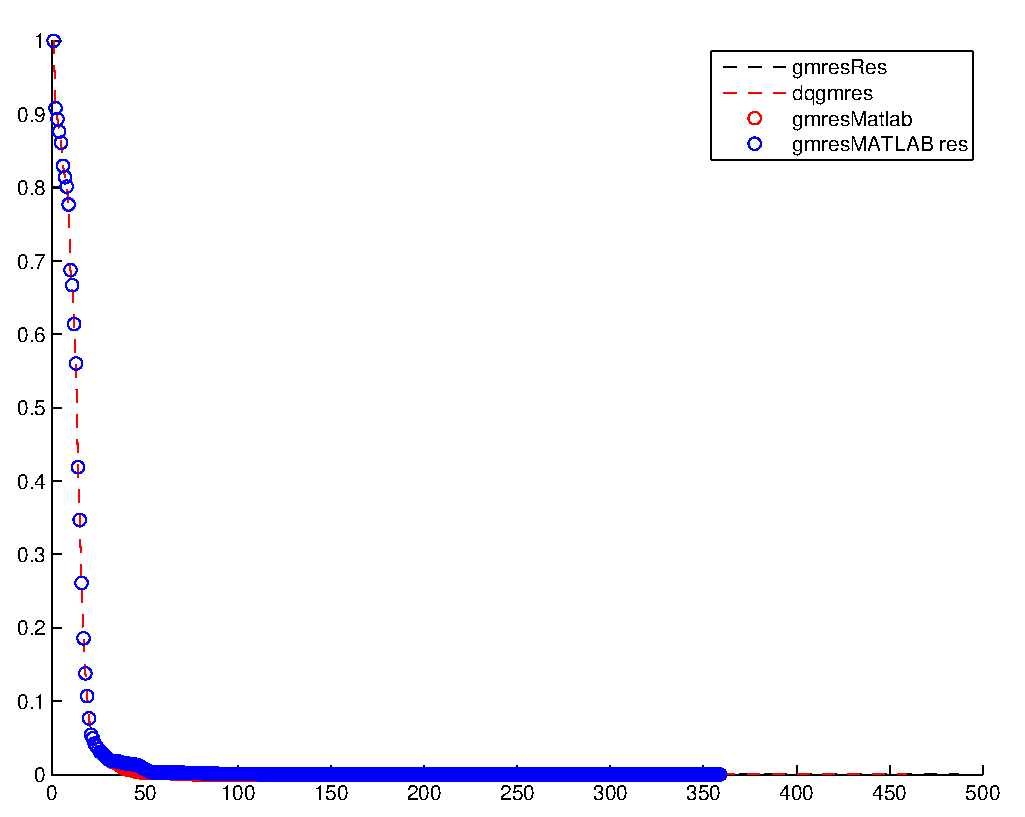
\includegraphics[scale=0.65]{diag.eps}
\end{center}
\newpage
\subsubsection*{Avec préconditionnement factorisation LU }
Ici, rien ne converge, toutes les méthodes stagnes et les résidus finaux sont trés grands. Le préconditionnement LU est en fait trés mauvais et inutile ici car on créé beaucoup de remplissage en le faisant, donc les préconditionneurs sont loins d'êtres facilement inversibles. On utilise ci-aprés une factorisation LU sans fill-in.
\subsubsection*{Avec préconditionnement factorisation LU sans fill-in}
On utilise la méthode ilu avec l'option 'no-fill' pour utiliser le fait que A soit creuse. Cette fois tout converge en trés peu d'itération :\\
gmresRES : 1.84e-8 en 51\\
gmresMRES : 9.39e-7 en 10\\
dqgmres : 3.37e-7 en 31\\
gmresM : 7.08e-7 en 31\\
\begin{center}
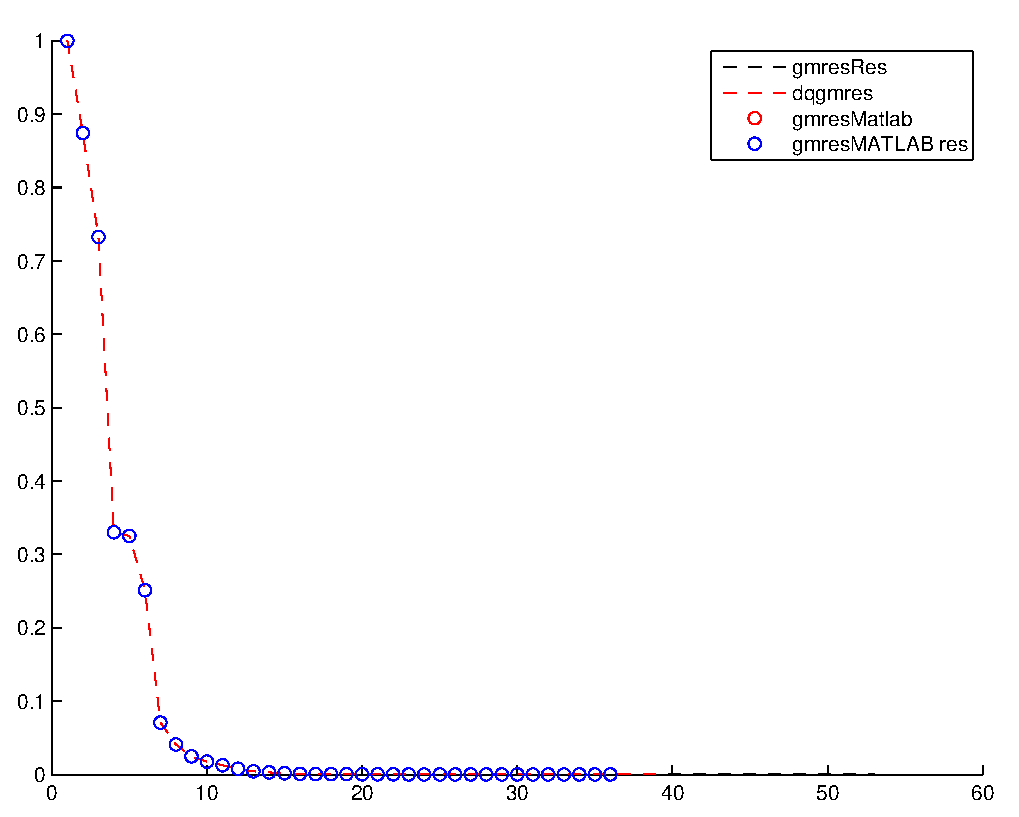
\includegraphics[scale=0.65]{lu.eps}
\end{center}
Ce préconditionnement est trés bon pour cette matrice. Il semble de plus peu coûteux pour la matrice A. En conclusion, ce préconditionneur est clairement le meilleur mais peut être pas le plus simple à calculer et à inverser (en comparaison avec la diagonale de A). On notera bien que les courbes des résidus entre gmresRES et gmresMRES sont bien identiques, donc que notre algorithme semble correct.
\newpage
\subsection{Test sur la fenêtre de dqgmres et gmresRES}
On effectue les tests avec $tol = 1e-6$, $maxit=600$, la matrice bfw398a, et le préconditionneur diagonal (si l'on prend le préconditionneur LU sans remplissage, le préconditionnement est trop bon et on ne voit pas de différence suiant la fenêtre). On fait varier la fenêtre sur redémarrage et la fenêtre d'orthogonalisation de dqgmres.
\subsubsection*{Sur gmresRES}
On prend des fenêtres qui valent 30, 60 et 100. Les résultats confirment ce à quoi on s'attendait : avec un fenêtre trop petite, la méthode s'éloigne trop de la solution et se met à stagner, et plus la fenêtre est grande, moins on a d'itération. Il faut donc prendre une fenêtre entre les deux, car si on la prend trop grande, la méthode n'a plus d'intêret puisqu'elle est presque équivalent à une gmres normale. Voici les résultats :
\begin{itemize}
\item pour 30 : résidu vaut 9.1e-4 et on dépasse \texttt{maxit}
\item pour 60 : résidu vaut 9.5e-7 et $iter=288$
\item pour 100 : résidu vaut 9.5e-7 et $iter=154$
\end{itemize}
\begin{center}
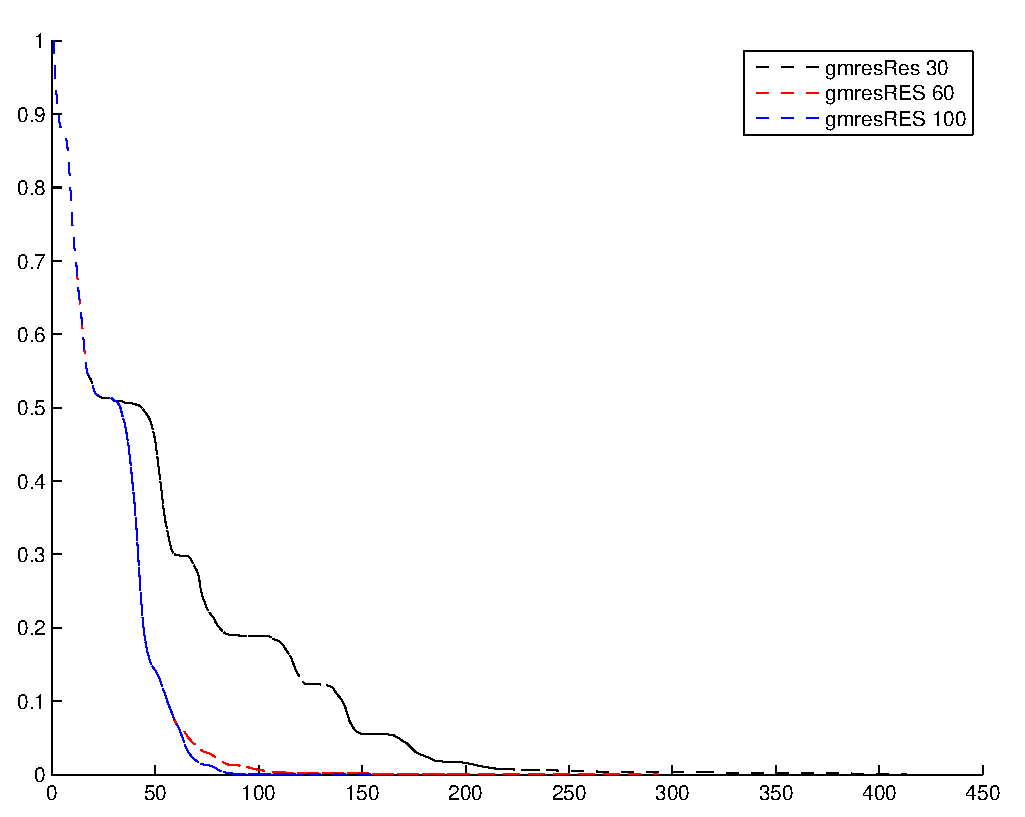
\includegraphics[scale=0.65]{res.eps}
\end{center}
\newpage
\subsubsection*{Sur dqgmres}
On prend cette fois des fenêtres qui valent 20, 30, 60 et 120. De même que précédemment, plus la fenêtre diminue, plus on perd d'informations sur  les vecteurs de la base, donc le résultat est moins précis, et parfois on ne converge pas:
\begin{itemize}
\item pour 20 : résidu vaut 1e-1 et on dépasse \texttt{maxit}}
\item pour 30 : résidu vaut 9e-7 et $iter=560$
\item pour 60 : résidu vaut 9e-7 et $iter=287$
\item pour 120 : résidu vaut 9e-7 et $iter=112$
\end{itemize}
\begin{center}
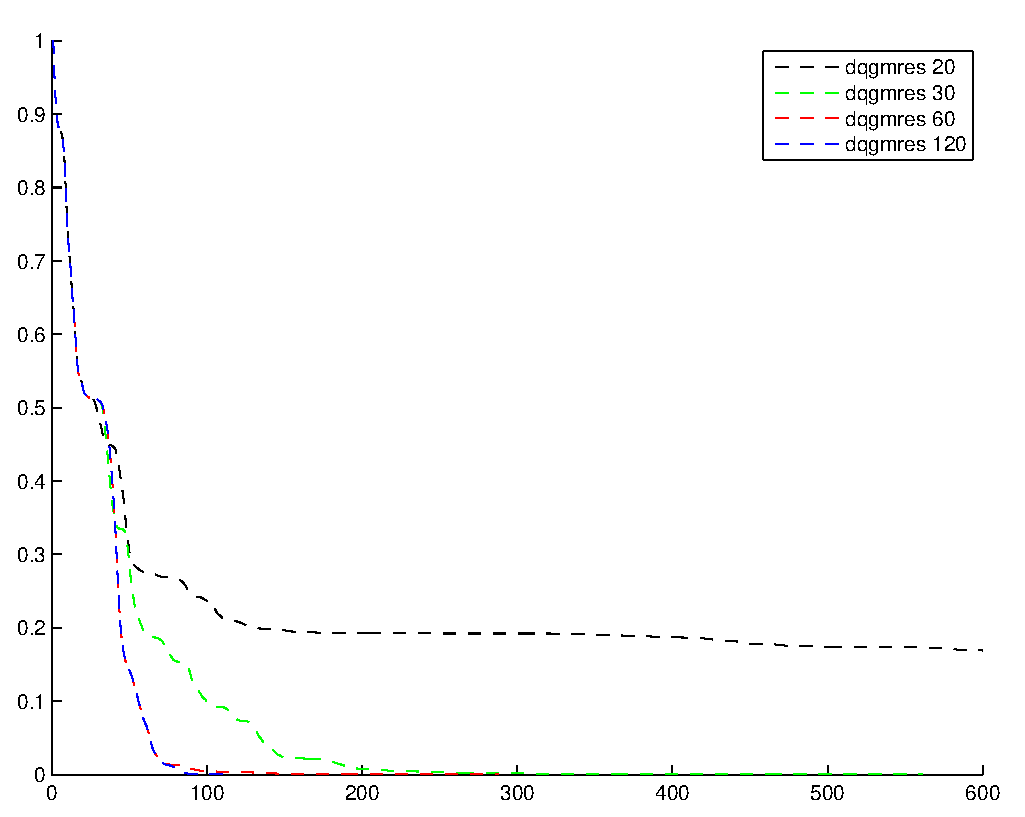
\includegraphics[scale=0.65]{dqgmres.eps}
\end{center}
\newpage
\subsection{Test sur la tolérance}
On effectue ce test sur la matrice bwm200, avec $maxit=600$ et avec un préconditionnement diagonal pour les mêmes raisons que précédemment, et avec dqgmres. La tolérance vaudra 1e-2, 1e-4, 1e-6 et 1e-8. Comme on peut s'en douter, plus la tolérance est faible, plus le nombre d'itération sera importante. Voici les résultats :
\begin{itemize}
\item 1e-2 : en 263 itérations en 0.74s
\item 1e-4 : 588 itérations en 15.7s
\item 1e-6 : non convergence, arrêt en 17s
\item 1e-8 : non convergence, arrêt en 17s
\end{itemize}
Les temps sont pris en moyenne sur plusieurs série de test : le temps d'exécution change à chaque fois un peu en raison des processus tournant en tâche de fond sur l'ordinateur.
\begin{center}
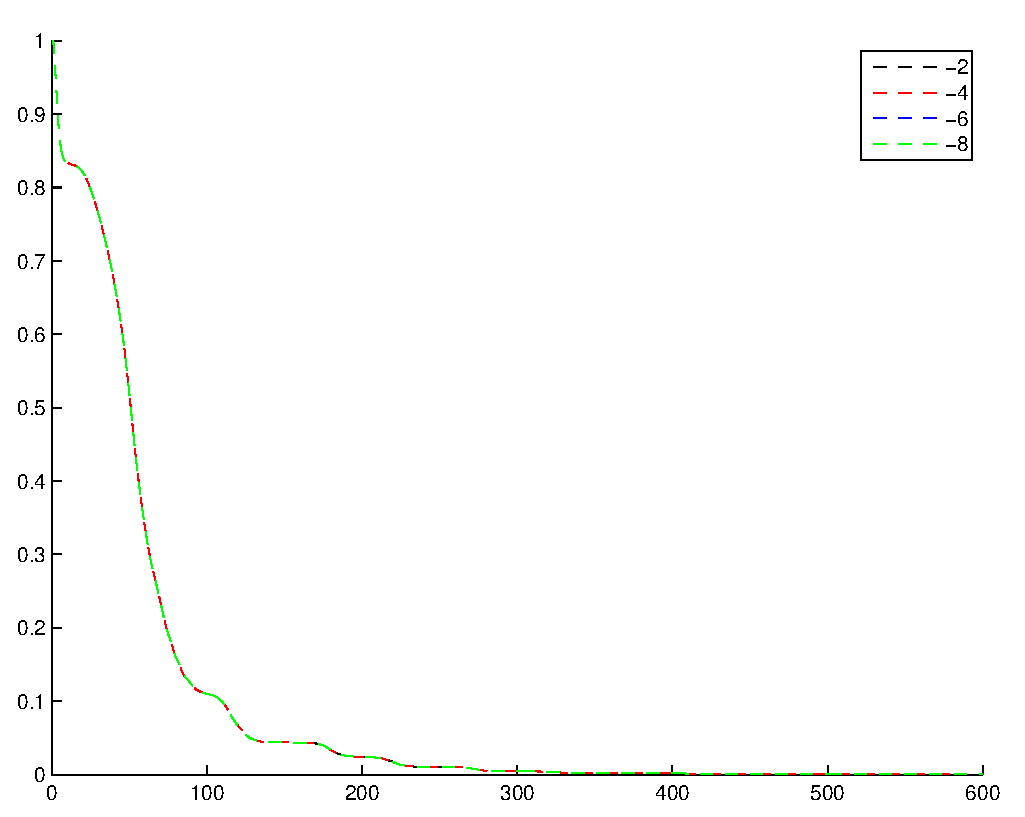
\includegraphics[scale=0.65]{tol.eps}
\end{center}
On remarque que de passer de 1e-2 à 1e-4 a multiplié par 20 le temps de calcul : ceci est du au fait que plus on fait d'itération dans dqgmres, plus on perd de l'information en orthogonalisant sur des vecteurs qui ne sont plus orthogonales par rapport aux précédents. Il faut donc bien choisir la tolérance dans dqgmres pour ne pas trop faire d'itération. 
